% This is the Reed College LaTeX thesis template. Most of the work 
% for the document class was done by Sam Noble (SN), as well as this
% template. Later comments etc. by Ben Salzberg (BTS). Additional
% restructuring and APA support by Jess Youngberg (JY).

\documentclass[12pt,twoside]{reedthesis}
\usepackage{graphicx,latexsym} 
\usepackage{amssymb,amsthm,amsmath}
\usepackage{longtable,booktabs,setspace} 
\usepackage[hyphens]{url}
\usepackage{rotating}
% \usepackage{natbib}
% Comment out the natbib line above and uncomment the following two lines to use the new 
% biblatex-chicago style, for Chicago A. Also make some changes at the end where the 
%bibliography is included. 
\usepackage{biblatex-chicago}
\bibliography{thesis}

% \usepackage{times} % other fonts are available like times, bookman, charter, palatino

\title{Yay Copepods}
\author{Ella Crotty}
% The month and year that you submit your FINAL draft TO THE LIBRARY (May or December)
\date{May 2025}
\division{Environmental Studies}
\advisor{Sam Fey}
%If you have two advisors for some reason, you can use the following
%\altadvisor{Your Other Advisor}
%%% Remember to use the correct department!
\department{Biology}
% if you're writing a thesis in an interdisciplinary major,
% uncomment the line below and change the text as appropriate.
% check the Senior Handbook if unsure.
\thedivisionof{The Established Interdisciplinary Committee for}
% if you want the approval page to say "Approved for the Committee",
% uncomment the next line
%\approvedforthe{Committee}

\setlength{\parskip}{0pt}

\begin{document}

  \maketitle
  \frontmatter % this stuff will be roman-numbered
  \pagestyle{empty} % this removes page numbers from the frontmatter

    \chapter*{Acknowledgements}
	I want to thank a few people.

% The preface is optional
% To remove it, comment it out or delete it.
    \chapter*{Preface}
	This is an example of a thesis setup to use the reed thesis document class.
	
    \chapter*{List of Abbreviations}
		You can always change the way your abbreviations are formatted. Play around with it yourself, use tables, or come to CUS if you'd like to change the way it looks. You can also completely remove this chapter if you have no need for a list of abbreviations. Here is an example of what this could look like:

	\begin{table}[h]
	\centering % You could remove this to move table to the left
	\begin{tabular}{ll}
		\textbf{ENSO}  	&  El Ni\~{n}o Southern Oscillation \\
		\textbf{OCNMS}  	&  Olympic Coast National Marine Sanctuary \\
	\end{tabular}
	\end{table}
	

    \tableofcontents
    \listoftables
    \listoffigures

% If your abstract is longer than a page, there may be a formatting issue.
    \chapter*{Abstract}
	The preface pretty much says it all.
	
	\chapter*{Dedication}
	You can have a dedication here if you wish.

  \mainmatter % here the regular arabic numbering starts
  \pagestyle{fancyplain} % turns page numbering back on

%The \introduction command is provided as a convenience.
%if you want special chapter formatting, you'll probably want to avoid using it altogether

    \chapter*{Introduction}
         \addcontentsline{toc}{chapter}{Introduction}
	\chaptermark{Introduction}
	\markboth{Introduction}{Introduction}
	% The three lines above are to make sure that the headers are right, that the intro gets included in the table of contents, and that it doesn't get numbered 1 so that chapter one is 1.

% \onehalfspacing
% \doublespacing
	
	

\section{Climate Change and Hypoxia in OCNMS}
	


\section{Copepods}

\begin{table}[htbp] 
	
	\caption[Seasonal classification of copepods]{Classification of copepods as cold-water (primarily occurring in the summer upwelling season) and warm-water (primarily occurring in the winter) according to NOAA Indicators, Peterson \& Keister 2003, Peterson and Miller 1977.}  % need to add in proper citations
	% square brackets --> Table of Tables. curly braces --> caption over the table.
	
	\begin{center} 
		\begin{tabular}{l l}  
			\toprule
			Species &  Group \\ 
			\midrule 
			\textit{Acartia clausii} 				& 	Cold-water 	 \\ 
			\textit{Acartia longiremis}	& Cold-water  \\
			\textit{Calanus marshallae}	& Cold-water  \\
			\textit{Centropages abdominales}	& Cold-water  \\
			\textit{Microcalanus pusillus}	& Cold-water  \\
			\textit{Pseudocalanus mimus} & Cold-water  \\
			\textit{Pseudocalanus spp.}	& Cold-water  \\
			\textit{Oithona similis}	& Cold-water/year-round  \\
			\textit{Acartia tonsa}	& Warm-water  \\
			\textit{Calanus pacificus}	& Warm-water  \\
			\textit{Calocalanus spp.}	& Warm-water  \\
			\textit{Calocalanus styliremis}	& Warm-water  \\
			\textit{Clausocalanus spp.}	& Warm-water  \\
			\textit{Corycaeus anglicus}	& Warm-water  \\
			\textit{Ctenocalanus vanus}	& Warm-water  \\
			\textit{Mesocalanus tenuicornis}	& Warm-water  \\
			\textit{Metridia pacifica}	& Warm-water  \\
			\textit{Paracalanus parvus}	& Warm-water  \\
			\textit{Paracalanus spp.}	& Warm-water  \\
			\bottomrule 
		\end{tabular}
	\end{center}
	\label{CopepodGroups} % to reference this table, write \ref{CopepodGroups}
\end{table}

\clearpage 

\section{Environmental DNA}

\section{Study Plan}


	
    \chapter{The First}
    	This is the first page of the first chapter. You may delete the contents of this chapter so you can add your own text; it's just here to show you some examples. 

   
   \section{\LaTeX Reference}
   
   \section{References, Labels, Custom Commands and Footnotes}
   It is easy to refer to anything within your document using the \texttt{label} and \texttt{ref} tags.  Labels must be unique and shouldn't use any odd characters; generally sticking to letters and numbers (no spaces) should be fine. Put the label on whatever you want to refer to, and put the reference where you want the reference. \LaTeX\ will keep track of the chapter, section, and figure or table numbers for you. 
   
   \subsection{References and Labels}
   Sometimes you'd like to refer to a table or figure, e.g. you can see in Figure \ref{subd2} that you can rotate figures . Start by labeling your figure or table with the label command (\verb=\label{labelvariable}=) below the caption (see the chapter on graphics and tables for examples). Then when you would like to refer to the table or figure, use the ref command (\verb=\ref{labelvariable}=). Make sure your label variables are unique; you can't have two elements named ``default." Also, since the reference command only puts the figure or table number, you will have to put  ``Table" or ``Figure" as appropriate, as seen in the following examples:
   
   As I showed in Table \ref{inheritance} many factors can be assumed to follow from inheritance. Also see the Figure \ref{subd} for an illustration.
   
   \subsection{Custom Commands}\label{commands}
   Are you sick of writing the same complex equation or phrase over and over? 
   
   The custom commands should be placed in the preamble, or at least prior to the first usage of the command. The structure of the \verb=\newcommand= consists of the name of the new command in curly braces, the number of arguments to be made in square brackets and then, inside a new set of curly braces, the command(s) that make up the new command. The whole thing is sandwiched inside a larger set of curly braces. 
   
   % Note: you cannot use numbers in your commands!
   \newcommand{\hydro}{H$_2$SO$_4$}
   
   In other words, if you want to make a shorthand for H$_2$SO$_4$, which doesn't include an argument, you would write: \verb=\newcommand{\hydro}{H$_2$SO$_4$}= and then when you needed  to use the command you would type \verb=\hydro=. (sans verb and the equals sign brackets, if you're looking at the .tex version). For example: \hydro
   
   \subsection{Footnotes and Endnotes}
   You might want to footnote something.\footnote{footnote text} Be sure to leave no spaces between the word immediately preceding the footnote command and the command itself. The footnote will be in a smaller font and placed appropriately. Endnotes work in much the same way. More information can be found about both on the CUS site.
   
   \section{Bibliographies}
   Of course you will need to cite things, and you will probably accumulate an armful of sources. This is why BibTeX was created. For more information about BibTeX and bibliographies, see our CUS site (\url{web.reed.edu/cis/help/latex/index.html})\footnote{\cite{reedweb:2007}}. There are three pages on this topic: {\it bibtex} (which talks about using BibTeX, at \url{/latex/bibtex.html}), {\it bibtexstyles} (about how to find and use the bibliography style that best suits your needs, at \url{/latex/bibtexstyles.html}) and {\it bibman} (which covers how to make and maintain a bibliography by hand, without BibTeX, at at \url{/latex/bibman.html}). The last page will not be useful unless you have only a few sources. There used to be APA stuff here, but we don't need it since I've fixed this with my apa-good natbib style file.
   
   \subsection{Tips for Bibliographies}
   \begin{enumerate}
   	\item Like with thesis formatting, the sooner you start compiling your bibliography for something as large as thesis, the better. Typing in source after source is mind-numbing enough; do you really want to do it for hours on end in late April? Think of it as procrastination.
   	\item The cite key (a citation's label) needs to be unique from the other entries.
   	\item When you have more than one author or editor, you need to separate each author's name by the word ``and'' e.g.\\ \verb+Author = {Noble, Sam and Youngberg, Jessica},+.
   	\item Bibliographies made using BibTeX (whether manually or using a manager) accept LaTeX markup, so you can italicize and add symbols as necessary.
   	\item To force capitalization in an article title or where all lowercase is generally used, bracket the capital letter in curly braces.
   	\item You can add a Reed Thesis citation\footnote{\cite{noble:2002}} option. The best way to do this is to use the phdthesis type of citation, and use the optional ``type'' field to enter ``Reed thesis'' or ``Undergraduate thesis''. Here's a test of Chicago, showing the second cite in a row\footnote{\cite{noble:2002}} being different. Also the second time not in a row\footnote{\cite{reedweb:2007}} should be different. Of course in other styles they'll all look the same.
   \end{enumerate}
   \section{Anything else?}
   If you'd like to see examples of other things in this template, please contact CUS (email cus@reed.edu) with your suggestions. We love to see people using \LaTeX\ for their theses, and are happy to help.
   
   \begin{table}[htbp] 
   	
   	\caption[Example]{Example Caption}  % need to add in proper citations
   	% square brackets --> Table of Tables. curly braces --> caption over the table.
   	
   	\begin{center}  % makes the table centered
   		\begin{tabular}{l l}  % column can be l, c, r, or p{width} to wrap, ex. p{1in}
   			\toprule % a horizontal line, slightly thicker than \hline, depends on the booktabs package
   			Column &  Column \\ % the first row of the table. Separate columns with ampersands and end the line with two backslashes. An environment begun in one cell will not carry over to adjacent rows.
   			\midrule % another horizontal line
   			\textit{1} 				& 	2	 \\ % another row
   			\bottomrule % yet another horizontal line
   		\end{tabular}
   	\end{center}
   	\label{Example} % to reference this table, write \ref{Example}
   \end{table}
   
   %% \clearpage ends the page, and also dumps out all floats. 
   %% Floats are things like tables and figures.
   %% If you want to make a table that is longer than a page, you will want to use the longtable environment. Uncomment the table below to see an example, or see our online documentation.
   
	% If you need a graphic or tabular material to be part of the text, you can just put it inline. If you need it to appear in the list of figures or tables, it should be placed in the floating environment. 
	
	And this is how you add a figure with a graphic:
	\begin{figure}[h]
	% the options are h = here, t = top, b = bottom, p = page of figures.
	% you can add an exclamation mark to make it try harder, and multiple
	% options if you have an order of preference, e.g.
	% \begin{figure}[h!tbp]
	   
	       \centering
	    % DO NOT ADD A FILENAME EXTENSION TO THE GRAPHIC FILE
	    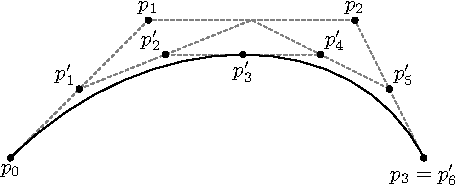
\includegraphics{subdivision}
	     \caption{A Figure}
	 \label{subd}
	\end{figure}

\clearpage %% starts a new page and stops trying to place floats such as tables and figures

\section{More Figure Stuff}
You can also scale and rotate figures.
 	\begin{figure}[h!]
	   
	       \centering
	    % DO NOT ADD A FILENAME EXTENSION TO THE GRAPHIC FILE
	    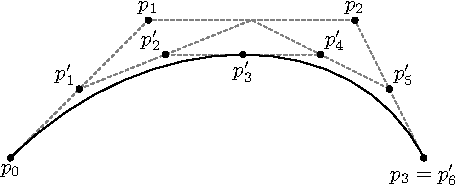
\includegraphics[scale=0.5,angle=180]{subdivision}
	    % if your figure shows up not where you want it, it may just be too big to fit. You can use the scale argument to shrink it, e.g. scale=0.85 is 85 percent of the original size. 
	     \caption{A Smaller Figure, Flipped Upside Down}
	 \label{subd2}
	\end{figure}
	
      \subsection{Common Modifications}
      The following figure features the more popular changes thesis students want to their figures. This information is also on the web at \url{web.reed.edu/cis/help/latex/graphics.html}.
    %\renewcommand{\thefigure}{0.\arabic{figure}} 	% Renumbers the figure to the type 0.x
    %\addtocounter{figure}{4} 						% starts the figure numbering at 4
    \begin{figure}[htbp]
    \begin{center}
   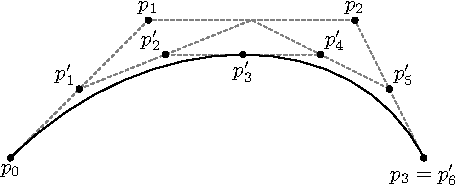
\includegraphics[scale=0.5]{subdivision}
    \caption[Subdivision of arc segments]{\footnotesize{Subdivision of arc segments. You can see that $ p_3 = p_6^\prime$.}} %the special ToC caption is in square brackets. The \footnotesize makes the figure caption smaller
    \label{barplot}
    \end{center}
    \end{figure} 

%If you feel it necessary to include an appendix, it goes here.
    \appendix
      \chapter{The First Appendix}


  \backmatter % backmatter makes the index and bibliography appear properly in the t.o.c...

% if you're using bibtex, the next line forces every entry in the bibtex file to be included
% in your bibliography, regardless of whether or not you've cited it in the thesis.
    \nocite{*}

% Rename my bibliography to be called "Works Cited" and not "References" or ``Bibliography''
 \renewcommand{\bibname}{Works Cited}

%\bibliographystyle{APA/apa-good}  % or
% \bibliography{thesis}
 % Comment the above two lines and uncomment the next line to use biblatex-chicago.
%\printbibliography[heading=bibintoc]

% Finally, an index would go here... but it is also optional.
\end{document}
